%% • The introduction must be dynamite. 
%% – The reader forms an oppinion of the work right from the start... 
%% • The introduction is an extension of the abstract. 
%% • Should be easy to read and understand 
%% • Should make it easy for anyone to tell
%% – What your paper is about 
%%   – What problem it solves
%%   – Why the problem and solution is interesting and relevant (motivation and context). Is it a long- outstanding problem?
%%   – What is new in your paper and how (much) does it improve on the strongest alternatives/previous work (include a few of the most relevant references here).

%% • Start the introduction with the motivation. Think in large contexts and don’t be afraid to be a poet.
%% • All implications, contributions and keypoints of your work must be included here.
%% • Make it very clear how your work will impact the future of Realistic image generation (will people use it?).
%% • If your work is pioneering, s-p-e-l-l i-t o-u-t.
%% • Briefly make it clear how you evaluate your method in the Results section.
%% • Make sure to explain where your method applies and where it does not apply (limitations).


\chapter{Introduction}

\chapterquote{Focus is a matter of deciding what things you're not
  going to do.}{John Carmack}


% Motivation

\textit{Rendering} is the process of converting a scene description into an
image and lies at the heart of \textit{computer graphics}. The ability to render
complex scenes realistically or distinctly is vital in several areas; computer
games, movies and even medical imaging. A scene is made up of models, which can
consist of several thousand geometric primitives, usually triangles. Information
about these triangles, or \textit{vertex attributes}, are stored at the vertices
and can be it's position, normal or color among other things.

% Rasterization and cube mapping

When real-time rendering is needed, the technique of choice for the last one and
a half decade has been \textit{rasterization}. In rasterization a geometric
primitives vertex attributes are mapped onto a \textit{raster}\footnote{A flat,
  2D grid.} and used to calculate the color of individual grid cells. This
technique is so popular in the gaming industry that processing units were
created specifically for rasterization, the \textit{Graphics Processing Unit} or
\textit{GPU} for short. Due to the industry's ever increasing demand for more
detailed models and effects, the GPU's have seen a massive increase in both
computational power and throughput over the last decade, as evidenced by
\reffig{fig:gflops}. Unfortunatly, even with all this power certain aspects of
rendering are still not easily solved by rasterization. \textit{Reflection} and
\textit{refraction} effects on non-flat surfaces are still notoriously hard to
recreate. The reason is that the reflection of complex objects can not easily be
mapped to a 2 dimensional grid, such as the raster. Reflections of complex
objects can be approximated by \textit{environment mapping} or \textit{cube
  mapping}, of which a short describtion can be found on
\reffig{fig:cubemap}. The trouble with cube mapping is that the scene must to be
rendered another 6 times, once for each side of the cube map. This can increase
the cost of rendering a scene by up to 6 times for each cube map
employed. Another shortcoming of cube mapping is that it doesn't support
\textit{self reflection}, since it is only the surrounding environment that is
rendered onto the map.

\begin{figure}
  \centering
  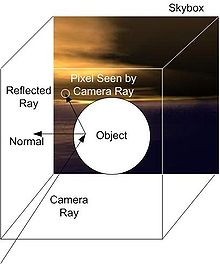
\includegraphics{Cube_mapped_reflection_example}

  \vspace{3mm}
  \parbox{9.5cm}{\caption[Cube mapping visualized.]{A visualization of
      cube mapping. The environment is rendered onto the sides of the
      cube and then mapped onto the sphere. The mapping is performed
      by using the calculated reflection vector as an index into the
      cube map.\\Image from
      http://en.wikipedia.org/wiki/Reflection\_mapping}\label{fig:cubemap}}
\end{figure}

% Ray tracing and comparing it to rasterization

Another technique for rendering is \textit{ray tracing}, which
eloquently solves reflection and refraction by tracing rays from the
eye and into the scene, spawning and tracing new reflection- and
refraction rays as needed when geometry is intersected. A comparisson
of cube mapping and ray tracing is given in
\reffig{fig:reflectingDragons}, where a reflecting stanford dragon has
been rendered with each technique. Notice how the ray traced dragons
backside reflects its neck, while the cube mapped version only
reflects the surrounding box. Advanced lighting techniques that
produce photorealistic images are also based on ray tracing. One such
technique is \textit{photon mapping}, which can accurately reproduce
the effects of lighting from reflective surfaces, caustics and color
bleeding.


% High cost used to make it unattractive for interactive scenes

The increased realisme that can be achieved with ray tracing does come
at a high computational cost, however, which has previously made it
unattractive for interactive applications or dynamic
scenes. Nonetheless, the recent increase in computational power
coupled with research into the area of \textit{interactive ray
  tracing} has yielded some incredible results.

\begin{figure}
  \centering
  \subfloat[A cube mapped reflecting dragon.]{
    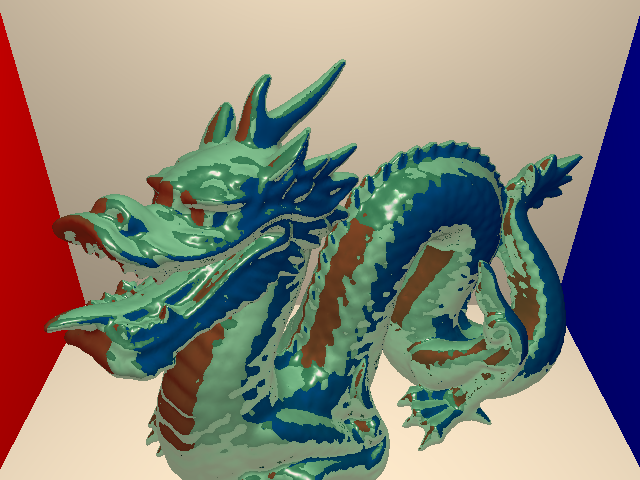
\includegraphics[width=7cm]{cubemappedDragon}
    \label{fig:cubeDragon}
  }
  \hspace{10pt}
  \subfloat[A ray traced reflecting dragon. Notice the self reflection
    on the back and inside the mouth.]{
    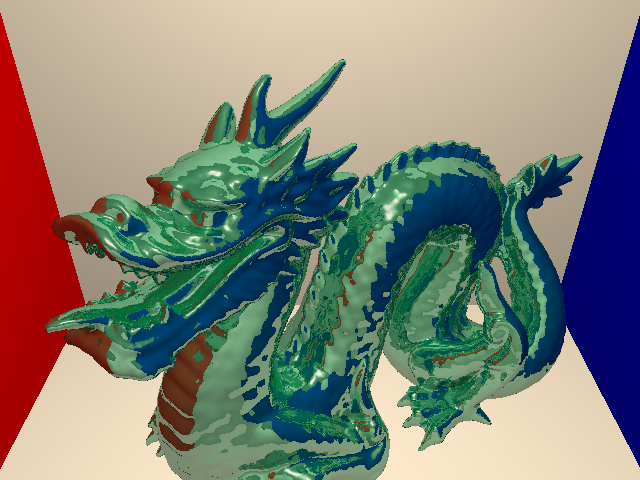
\includegraphics[width=7cm]{semiReflectingDragon}
    \label{fig:rayReflectingDragon}
  }
  \caption[Cube mapping vs raytracing for reflections.]{An example of
    the difference between using cube mapping or raytracing for
    reflections.}
  \label{fig:reflectingDragons}
\end{figure}


% What I will show, doing it dynamically, which is interesting for
% games and movie development

In this thesis I will examine \textit{ray tracing of dynamic scenes},
which could become an interesting alternative to rasterization in the
gaming industri and certainly is interesting for 3D artists working on
large screen movie productions, where ray tracing is already used for
\textit{CGI}\footnote{Computer-generated Imagery} effects and the
artists need fast visual feedback when rearranging the scene.


% We need Acceleration stuctures for ray tracing to achieve this

To improve the performance of ray tracers, several acceleration
structures have been developed. The most popular structures are
\textit{hierarchical data structures}, such as trees, and the ray
tracers that traverse them are called \textit{hierarchical ray
  tracers}. When the ray of a hierarchical ray tracer traverses a
hierarchical data structure it is in search of the nearest leaf node,
which contains references to the geometry nearest to the ray. If the
ray finds that it did not see, or intersect, any of the geometry in
the current leaf node, it advances beyond the leaf and performs
another traversal of the structure.

The structure employed in this thesis is the \textit{kd-tree}, a
binary, space partitioning tree-structure, which recursively
subdivides $k$-dimensional geometry by splitting it with \textit{axis
  aligned splitting planes}. Each interior node in the tree contains a
splitting plane and a reference to the location of its left and right
children, while the leafs contain references to the geometry
associated with them. An example of a subdivided scene and the
corrosponding tree can be seen in \reffig{fig:noEmptySpaceExample}. If
a leaf node, $n$, is split by a splitting plane, the geometry
associated with $n$ must be associated with its two newly constructed
child nodes. A kd-tree's quality is related to the choice of splitting
planes and a lot of computational power can go into finding optimal
splitting planes, as there are infinitely many possible
\textit{splitting plane candidates}, or \textit{split candidates}, to
consider. In a high quality kd-tree, splitting planes have been chosen
such that spatially close geometry are allocated into the same
subtree. Choosing a splitting plane for a node is the topic of
\refsection{sec:splittingPlane}. In order to facilitate dynamic
scenes, the data structure must also be dynamic. In the case of
kd-trees, this means completely rebuilding it from scratch. Because of
this the algorithm for creating the kd-tree needs to be very fast, and
might have to sacrifice tree quality for improved construction speed.


% Why do it on the GPU, yes why indeed? Leaves the CPU free to do
% other things than rendering.

As observed above, the GPU's have grown quite powerful over the last
decade, and since the introduction of programmable GPU's and NVIDIA's
\textit{CUDA}\footnote{Compute Unified Device Architecture.}
framework, many algorithms have been succesfully ported to utilize the
resources of the GPU. I will be doing the same in this thesis and use
the GPU to accelerate the creation of data structures and ray tracing
them. The most compelling reason to do this, is that it leaves the CPU
free to handle other aspects of a graphics application, such as game
logic and networking in a computer game.



\section{Goals}

In this thesis the goal is not to produce images of photorealistic
quality, or create an interactive ray tracer for dynamic
scenes \footnote{This goal alone can be achieved trivially by
  reducing the complexity of the scene or lowering the resolution.}
Instead this thesis will explorer ray tracing acceleration structures,
specifically the kd-tree, and it's impact on ray tracing efficiency
for dynamic scenes.

There are 3 ways to optimize ray tracing with respect to dynamic
scenes. 

\begin{enumerate}
  \item \textbf{Create a faster ray tracer -} Several optimizations
    exists that improve the speed of a ray tracer independently of the
    underlying acceleration stucture. Such optimizations will be
    discussed in \refsection{sec:hierarchicalTraversal}.
  \item \textbf{Building a higher quality acceleration structure -} An
    acceleration structure of higher quality can reduce the time it
    takes the ray tracer to find the nearest intersecting point
    between a ray and the scene. Algorithms for producing kd-tree's
    of different quality is the topic of
    \refsection{sec:splittingPlane}.
  \item \textbf{Build the acceleration structure faster -} In a
    dynamic scene, the acceleration structure may need to be rebuild
    each time the scene is rendered. Being able to rebuild it fast is
    therefore crucial. One way to ensure a faster reconstruction is by
    reducing the time spend deciding where to place the splitting
    plane, which can result in trees of lower quality.
\end{enumerate}

The main topic in this thesis is the relationship between tree quality
and construction speed. I will investigate different parts of the
kd-tree construction phase for dynamic scenes and wether sacrificing
tree quality for speed is worthwhile in dynamic scenes, or if the ray
tracing phase suffers a too high performance penalty from traversing a
lower quality tree.

The two parts of the kd-tree creation phase that I will investigate is
the choice of splitting plane, \refsection{sec:splittingPlane}, and
how geometry is associated with child nodes after a split,
\refsection{sec:splittingSchemes}.

The constructed kd-trees will be evaluated in \refchapter{chp:results}
by how fast they can be constructed and how efficiently a ray tracer
can traverse them and render the test scenes. The goal of this thesis
is then to find a kd-tree configuration that minimizes the total time
spend creating and traversing the structure and perhaps show that
there is a tradeoff between construction speed and tree quality.

To give a fair comparison of the time spend ray tracing and the time
spend building the data structure, I will need to create an optimized
ray tracer. This optimization is important as the optimized ray tracer
can render a scene up to XX\% faster than the basic implementation,
without increasing the computational cost of the kd-tree construction
phase. An entire chapter, \refchapter{chp:rayTracing}, is therefore
devoted to ray tracing optimization, but the topic is secondary to
kd-trees and merely included for testing purposes.

Given the added overhead of continuously rebuilding an acceleration
structure, an interesting question is wether or not we even need
it. In \refsection{sec:exhaustive} I therefore present an
\textit{exhaustive ray tracer}, which intersects every ray with every
triangle. The exhaustive ray tracer will be compared to the
hierarchical ray tracers and hopefully motivate the continued use of
acceleration structures for dynamic scenes.


%% The kd-tree used in this thesis to accelerate ray tracing is based on
%% the implementation described by \zhou. In this thesis I extend their
%% kd-tree construction with 2 new algorithms for deciding where to place
%% the splitting plane. Both algorithms will produce kd-trees
%% substantially faster than the original method proposed in \zhou, but
%% may reduce the quality of the tree, thus potentially increasing ray
%% tracing time. An improvement to the tree quality in \zhou{} is
%% \textit{empty space maximization}, which places empty nodes in the
%% tree and thus facilitates an early out option for a ray tracer, as
%% described in \refsection{sec:emptySpace}. I shall investigate wether
%% or not the added computational cost of this optimization is worthwhile
%% in dynamic scenes.

%% Once a node in the kd-tree has had its splitting plane's position
%% decided and its left and right child nodes created, the geometry needs
%% to be assigned to these new nodes. The most common technique is
%% \textit{triangle splitting}, where a triangle is split and up to 3 new
%% triangles are created. In \refsection{sec:splittingPlane} I
%% investigate 2 different approaches, in which the triangle is not split
%% into new triangles, but instead merely assigned to the child node it
%% overlaps. Since a triangle can maximally be assigned once to each
%% child node, this procedure will construct up to 2 new triangles per
%% original triangle and should therefore create smaller kd-trees.

%% However, given the overhead of keeping the acceleration structure
%% updated, I present in this thesis an exhaustive ray tracer, which will
%% intersect every ray with every triangle. While the structure of an
%% exhaustive ray tracer fits the GPU architecture better than a
%% hierarchical ray tracer, as we shall see in
%% \refsection{sec:exhaustive}, the overall performance seen in
%% \refchapter{chp:results} should motivate the continued use of
%% acceleration structures.

%% Different methods for creating KD-trees will be evaluated based on the
%% total time spend in to the kd-tree creation phase and the time
%% spend in the ray tracing phase.

%% \fixme{Ray tracing optimization will take up a large part of the
%%   thesis, but is secondary to the kd-trees and merely there to test
%%   them.}

%% To give a fair comparison of the time spend ray tracing and the time
%% spend building the data structure, I will need to create an optimized
%% ray tracer. Optimizing the ray tracer for this comparison is
%% important, since the optimized implementation is up to 80\% faster
%% than the basic implementation, with no added cost or logic to the
%% kd-tree creation phase. Optimizations to the ray tracer will be
%% inspired by the work done by \horn , but also include investigation of
%% optimal ray/triangle intersection algorithms, an improvement inspired
%% by empty space maximization during kd-tree creation and simply
%% structuring the rays in a manner that favors SIMD execution.

%% Ray tracing optimizations will simply be evaluated based on time saved
%% during ray tracing. Optimizations will be based on improving the
%% worst case scenarios, i.e. long rays shooting towards the center of
%% the scene.

\section{Overview}

The thesis is structured as follows:

% Previous work

The next section details previous work in the area of ray tracing and
kd-tree construction. This includes a brief history of when ray
tracing was introduced, aswell as key points in time for different
acceleration structures. The last part of this section will focus on
kd-trees and ray tracing on graphics hardware. Changes in this thesis
compared to previous work in the area are also outlined in this
section.

% Understanding CUDA

A chapter will then introduce NVIDIA's CUDA framework. Here I will
describe its thread and memory model. I will then go on to describe a
new primitive as proposed by Sengupta et al.\citebook{Sengupta:2007},
which will be much needed when assigning triangles to leaf nodes after
a split. Finally this section will focus on optimization techniques
specific to CUDA. These will be applied incrementally in a case study
of a global minima algorithm.

% kd-trees

\refchapter{chp:kdTrees} is then devoted to discussing kd-trees. The
first part of this section deals with the general kd-tree construction
algorith. Here I will present several algorithms for choosing the
splitting plane and discuss 3 different algorithms for associating
triangles with child nodes. The second part of the section deals with
the actual implementation of kd-trees on a GPU.

% raytracing

Having introduced kd-trees, the next chapter will deal with the
algorithms for traversing such trees and ray tracing the scene. Here
several optimizations to a basic heirarchical ray tracer will be
discussed and incrementally added. First though, an exhaustive ray
tracer is presented and will be used in the Results chapter to
motivate the use of hierarchical data structures. This section also
includes a discussion of 2 triangle intersection algorithms with
respect to performance on the graphics hardware.

% Results

% Conclusion

% Future work
